\paragraph{Caso d'uso UC7.2.3:  Visualizza Informazioni Personali}
\label{UC7_2_3}
\begin{figure}[ht]
	\centering
	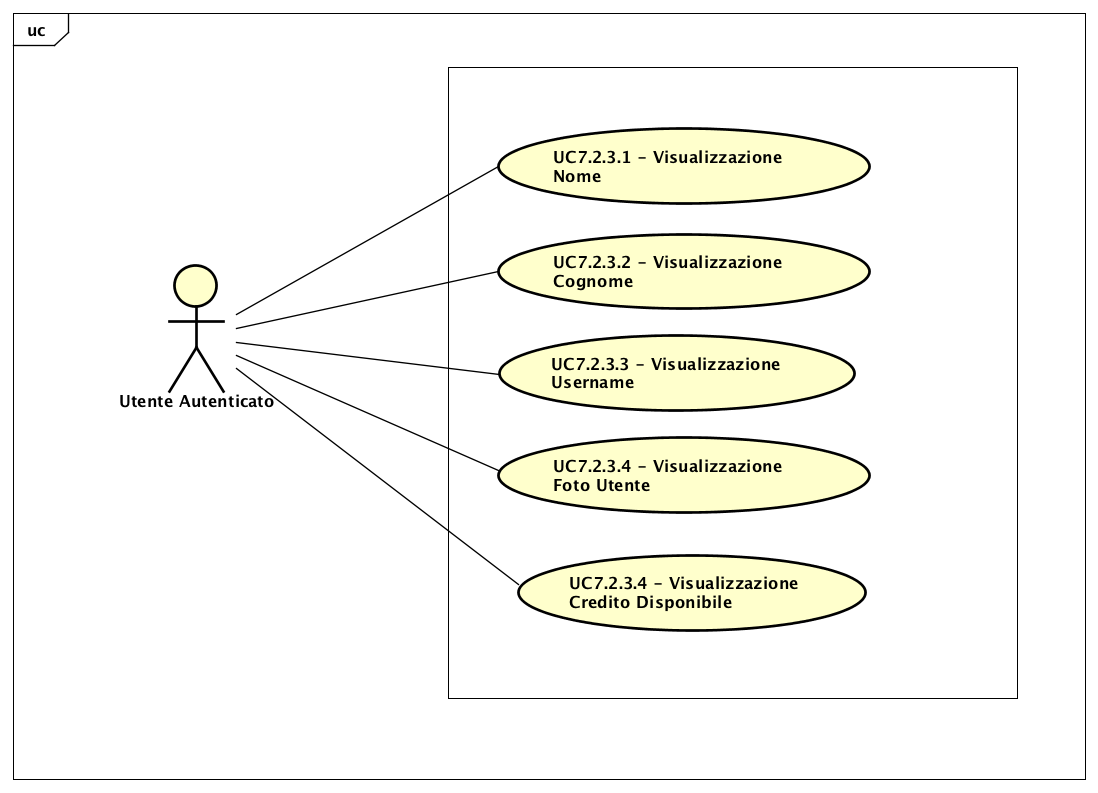
\includegraphics[scale=0.45]{UML/UC7_2_3.png}
	\caption{UC7.2.3: Visualizza Informazioni Personali}
\end{figure}

\FloatBarrier
\begin{tabular}{ l | p{11cm}}
	\hline
	\rowcolor{Gray}
	 \multicolumn{2}{c}{UC7.2.3:  VIsualizza Informazioni Personali} \\
	 \hline
	\textbf{Attori} & Utente Autenticato \\
	\textbf{Descrizione} & Gli utenti visualizzano le informazioni del proprio Profilo Utente\\
	\textbf{Pre-Condizioni} & L'utente e' nella schermata di gestione Profilo\\
	\textbf{Post-Condizioni} & L'utente ha modificato con successo il proprio Cognome \\
	\textbf{Scenario Principale} & 
	\begin{enumerate*}[label=(\arabic*.),itemjoin={\newline}]
		\item L'utente puo' Visualizzare il Nome (UC7.1.3.1)
		\item L'utente puo' Visualizzare il Cognome (UC7.1.3.2)
		\item L'utente puo' Visualizzare l'Username (UC7.1.3.3)
		\item L'utente puo' Visualizzare la Foto Utente (UC7.1.3.4)
		\item L'utente puo' Visualizzare il suo Credito Disponibile (UC7.1.3.4)
	\end{enumerate*}\\
\end{tabular}
